\cleardoublepage
\section{I2V生成}
\subsection{整体框架}

为了研究参考图像生成视频的效果,我们首先考虑将固定的参考图像作为视频的首帧来进行I2V(Image-to-Video)任务的训练方式。该框架通过将图像信息引入视频生成过程,能够使生成的视频更好地与输入图像的主题相关联,从而提升视频生成的准确性与多样性。\

\subsection{具体实现}

在具体实现中,首先给定一张参考图像,我们需要通过VAE(变分自编码器)编码将图像转换为潜在变量(latent)。将图像信息转化为潜变量后,可以在潜变量空间进行处理,这样可以有效降低训练的速度和显存消耗,提升生成效率。

目前,常见的I2V训练策略有以下两种:

\textbf{首帧替换策略}:这种策略将训练视频的第一帧替换为图像的潜在表示(latent)。在每次训练时,图像的潜在表示(\text{image\_latent})不会加入噪声。因此,在注意力计算(attention)过程中,视频的token能够与图像信息进行交互,从而使生成的视频主题与图像内容高度相关。
\begin{figure}[htbp]
    \centering
    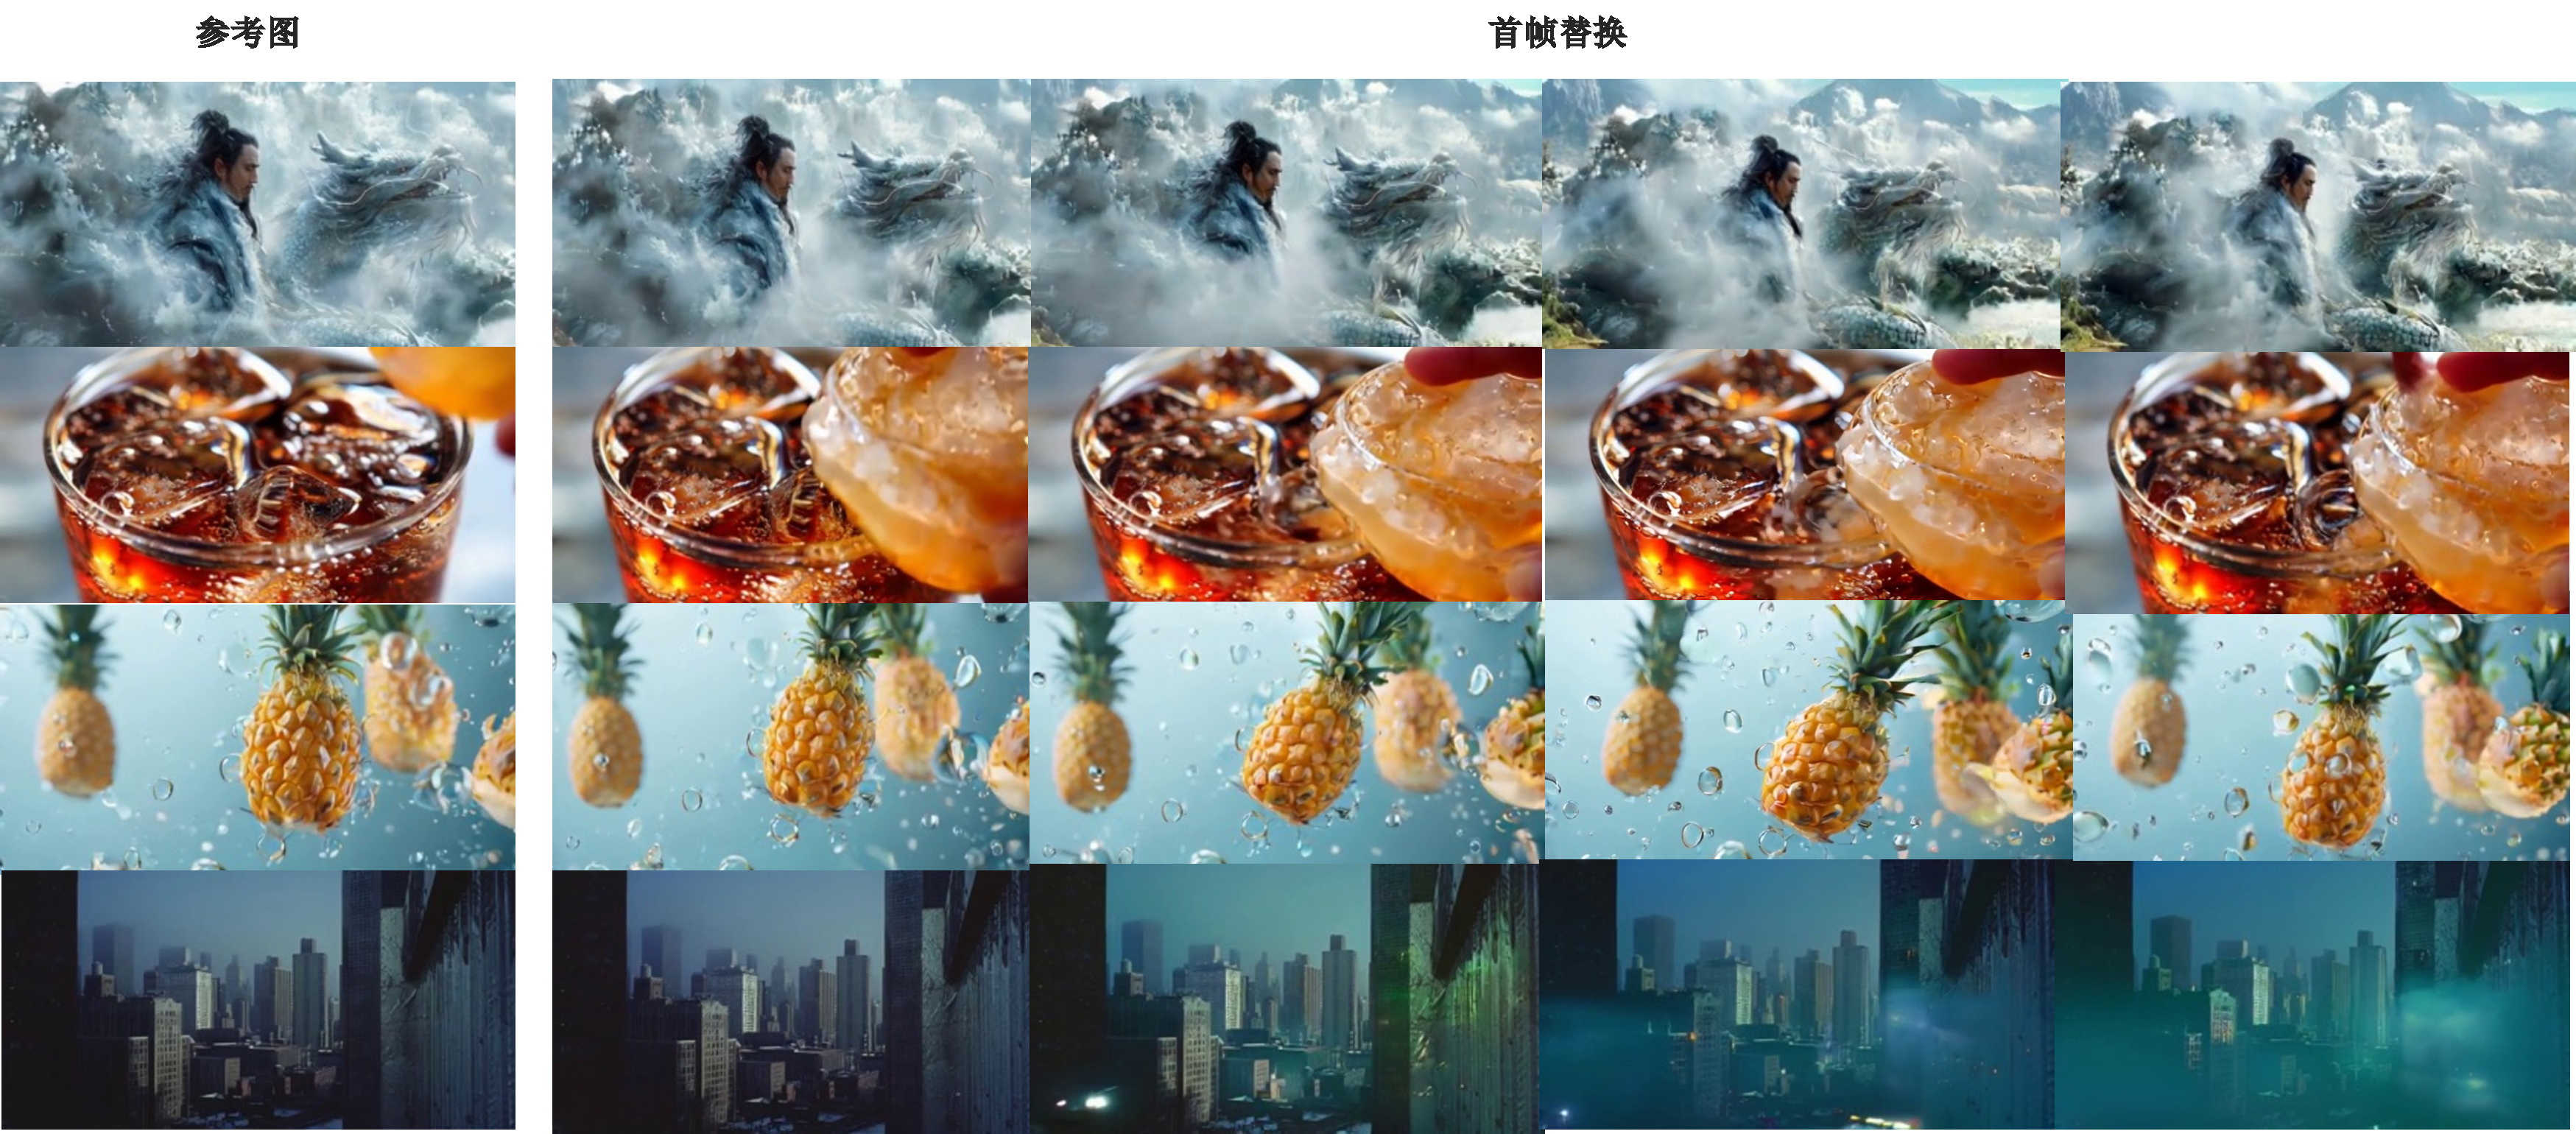
\includegraphics[width=0.8\textwidth]{final/I2V_1.pdf}
    \caption{\textbf{首帧替换策略生成结果}
    }
    \label{I2V_1}
\end{figure}

由图\ref{I2V_1} 可以发现首帧替换策略生成case基本符合要求,即视频生成主体一致性保持良好,没有出现主体漂移和人物失真等常见现象。


\textbf{参考帧拼接策略}:在这种策略下,训练时将图像的潜在表示(latent)拼接到视频的最后一帧的潜在表示中,之后再传入Transformer模型进行处理。\
在位置编码时,需要特别标明最后一帧不是正常的视频帧,而是参考图像的潜在表示,这里是直接让拼接上去的图像帧的位置编码等于首帧的位置编码,从而达到I2V的效果。\
这种方法通过在时间维度上拼接图像潜在信息,能够在视频生成过程中结合图像的视觉特征,使生成的视频更好地体现出参考图像中的关键元素。
\begin{figure}[htbp]
    \centering
    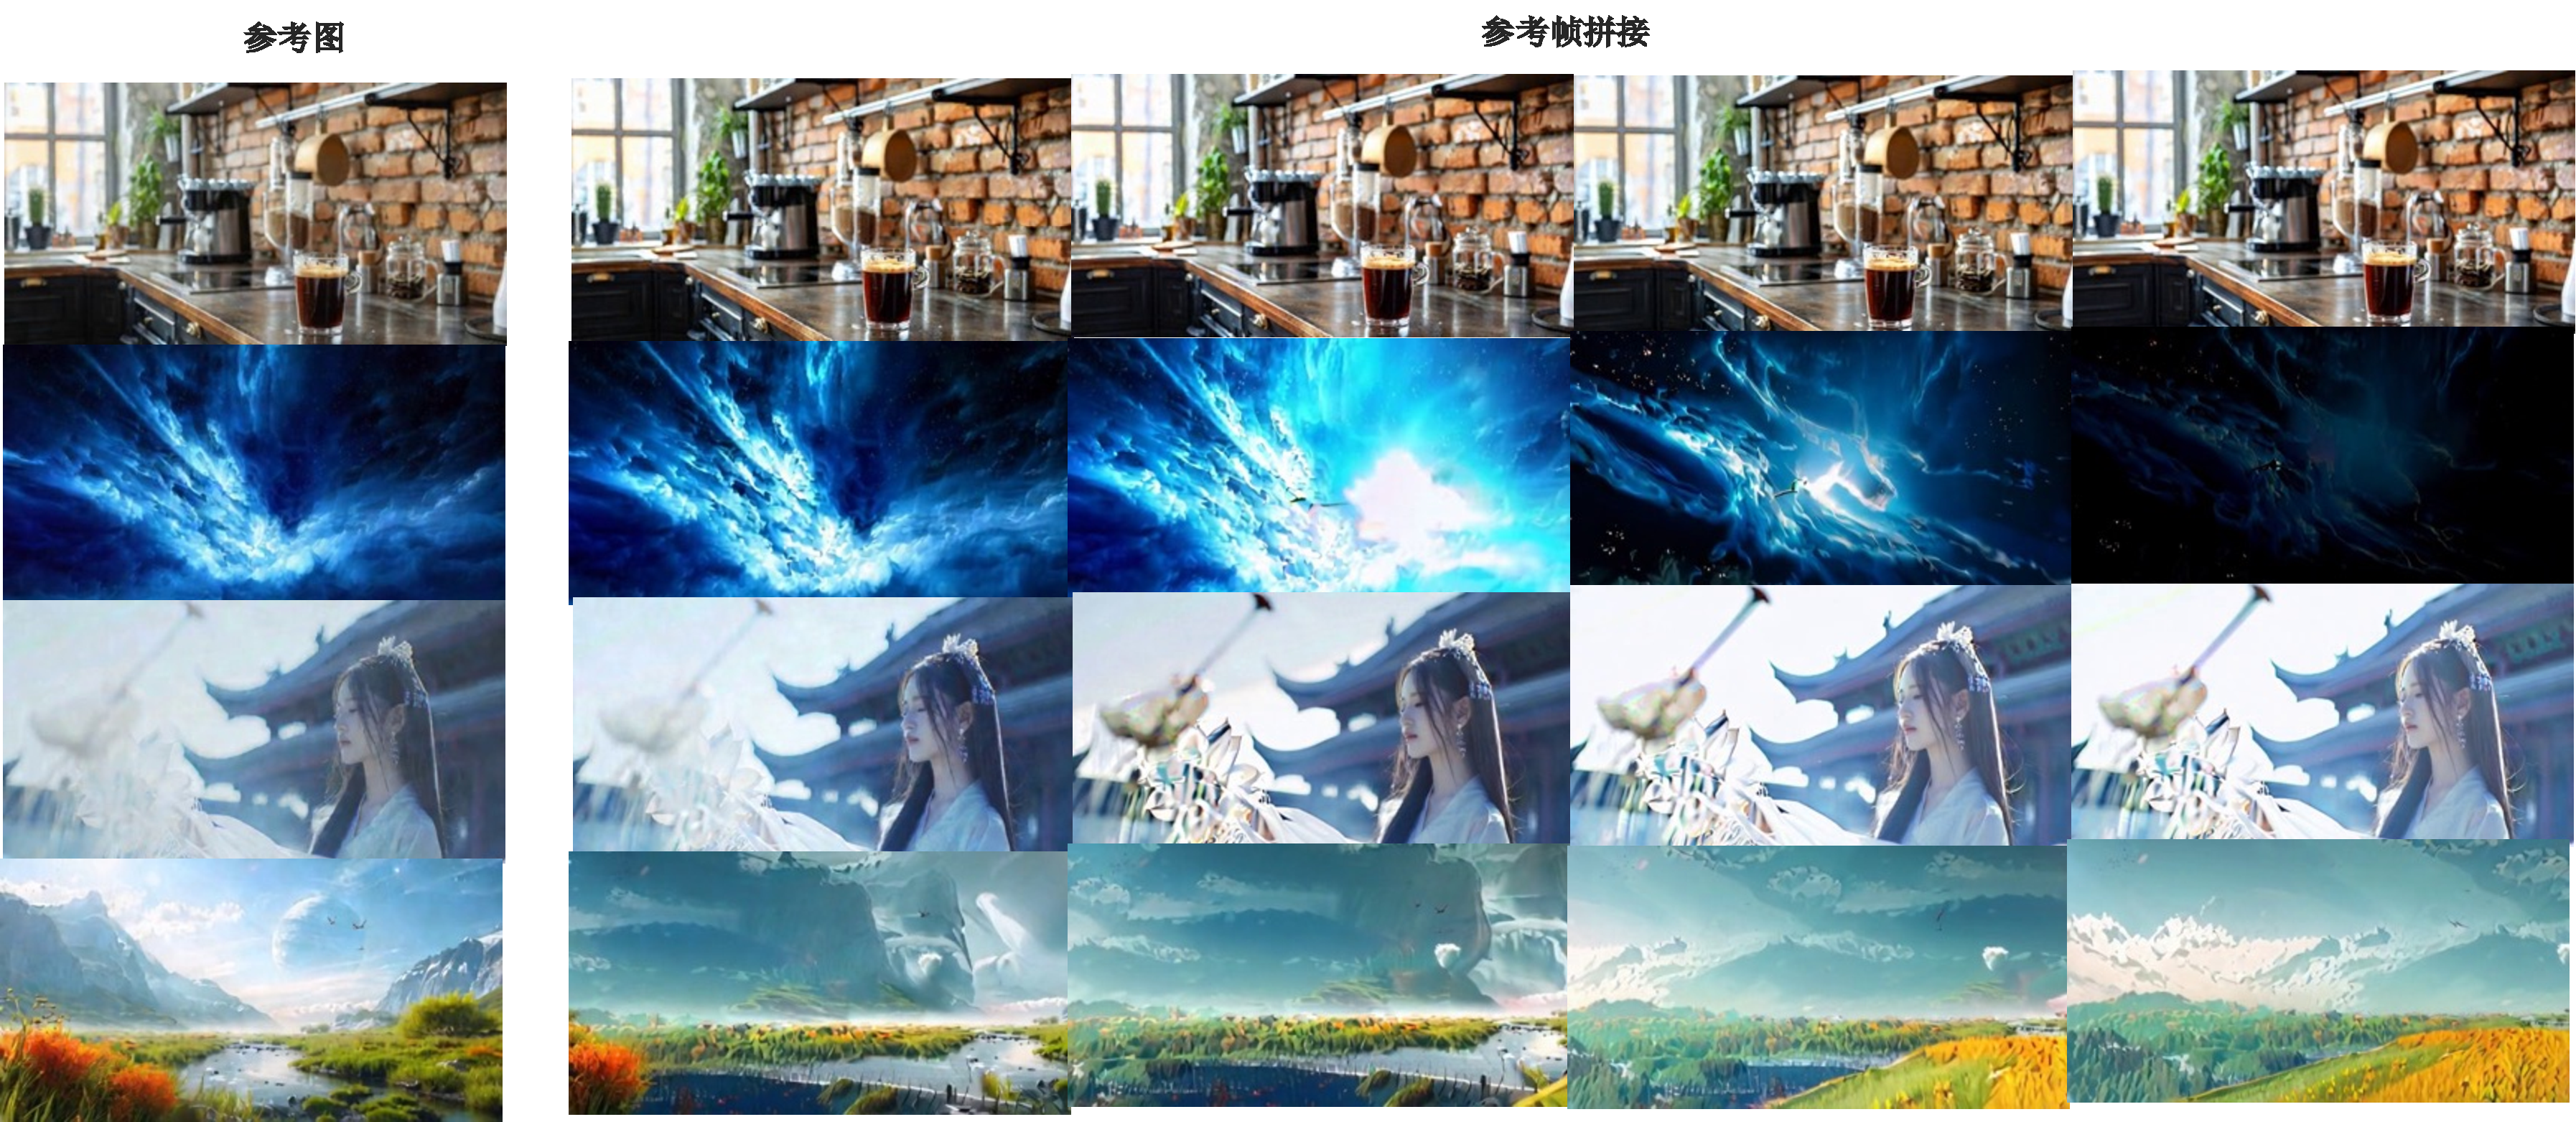
\includegraphics[width=0.8\textwidth]{final/I2V_2.pdf}
    \caption{\textbf{参考帧拼接策略生成结果}
    }
    \label{I2V_2}
\end{figure}
由图\ref{I2V_2} 可以发现参考帧拼接生成结果在一些例子上运动幅度很小,如针对女性手持花束,并且摇摆花束的例子,视频中摇动的幅度很小。但是也保持了生成视频中的主体人物和参考图片内容基本一致,但是文本响应度有待提升。

\begin{figure}[htbp]
    \centering
    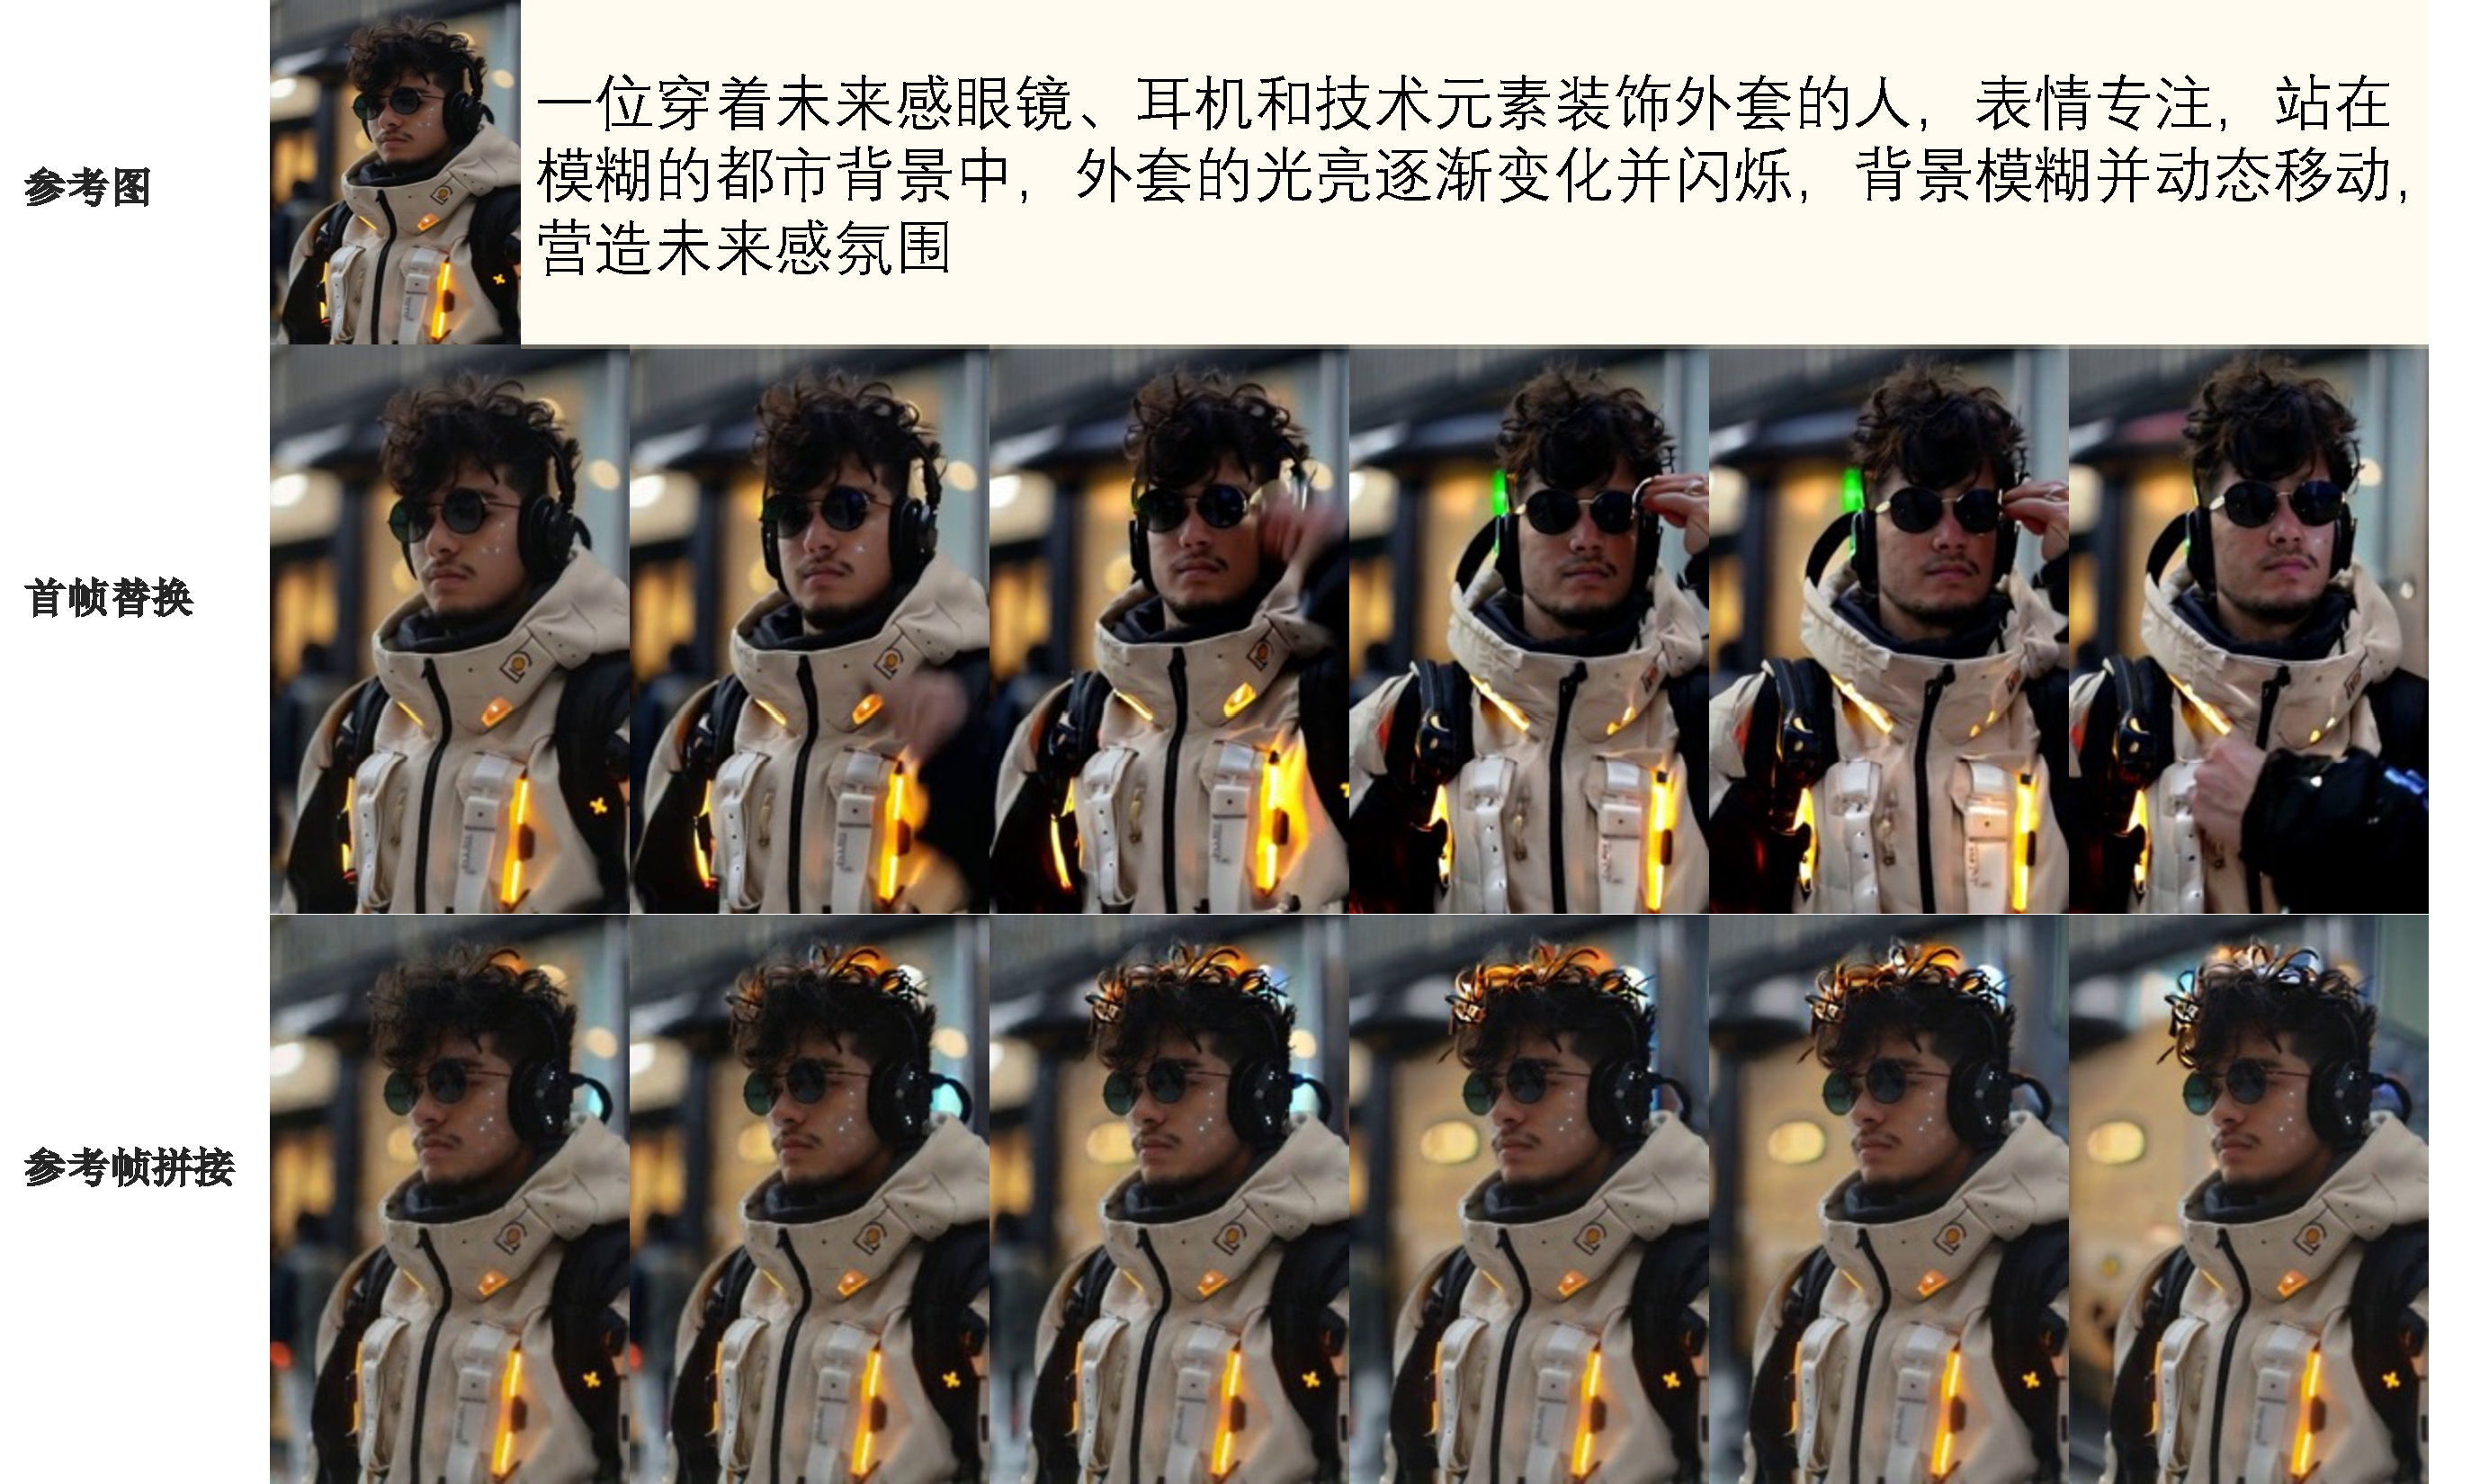
\includegraphics[width=0.8\textwidth]{final/I2V_4.pdf}
    \caption{\textbf{对比两种不同训练方式生成结果}
    }
    \label{I2V_4}
\end{figure}

\begin{figure}[htbp]
    \centering
    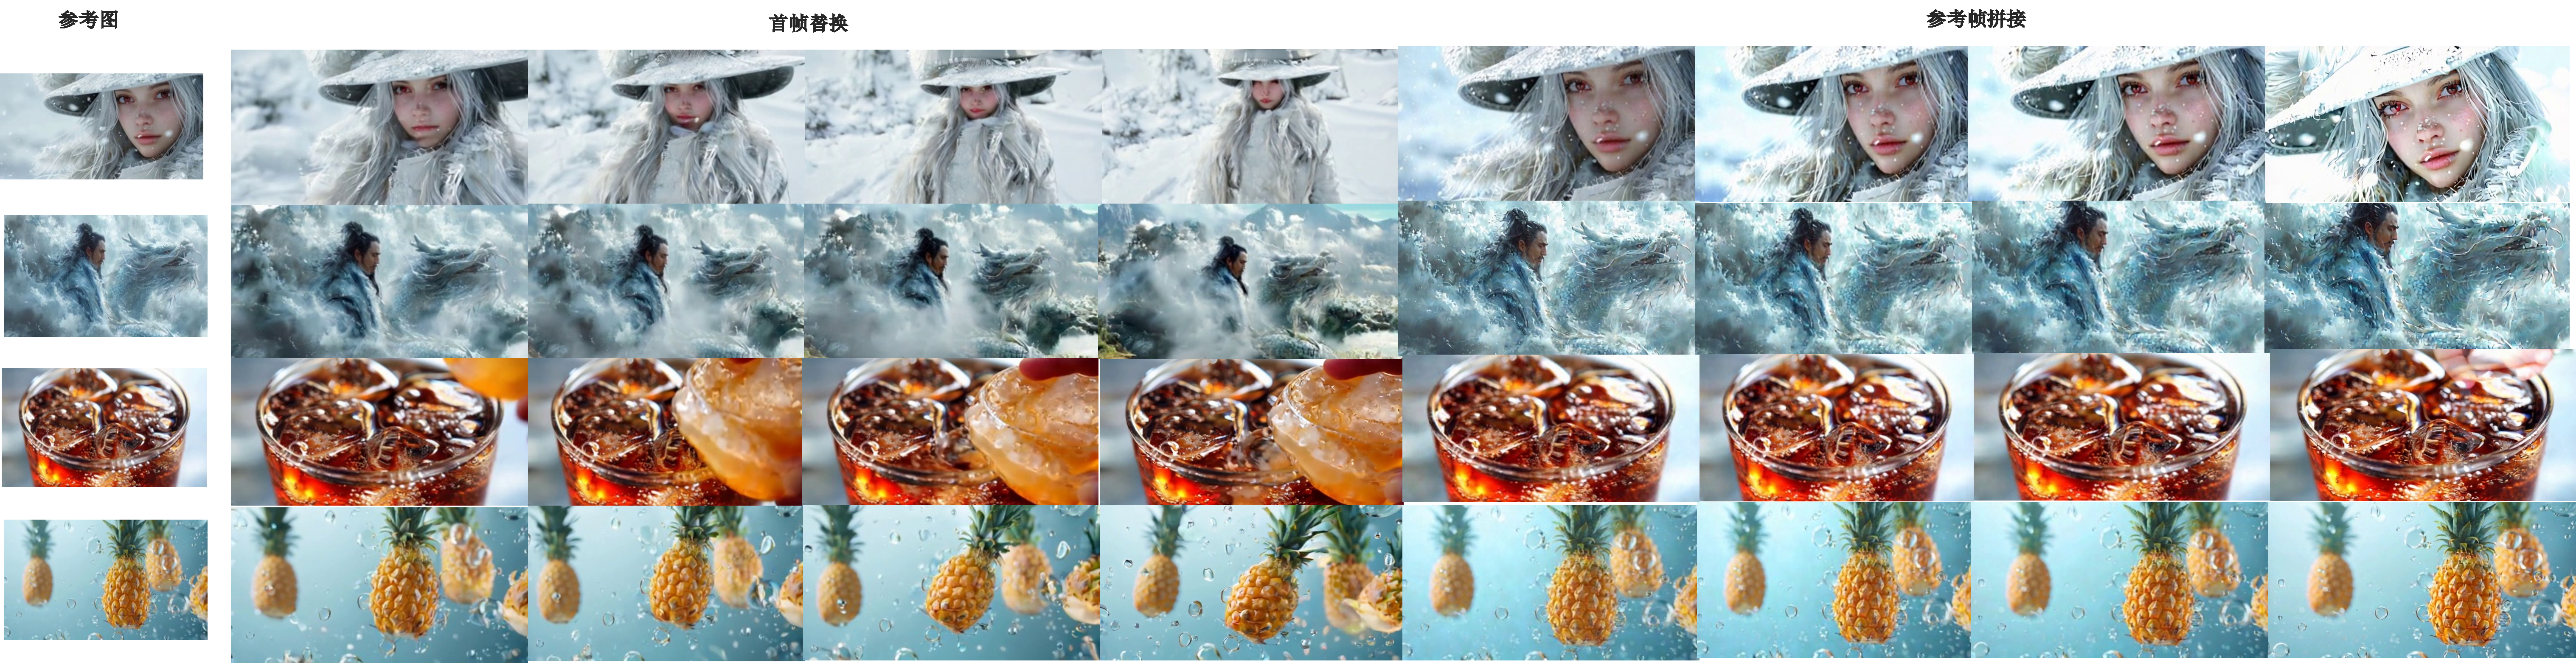
\includegraphics[width=0.8\textwidth]{final/I2V_3.pdf}
    \caption{\textbf{对比两种不同训练方式生成结果}
    }
    \label{I2V_3}
\end{figure}

根据对比图\ref{I2V_3} 可以明显看到对于给定的prompt `Red-eyed woman in snow with serene and mysterious atmosphere, melting snow`(一位红眼银发的女性站在雪地中,雪花附着在她的衣服和帽子上,气氛宁静神秘,雪慢慢融化), `Man with long hair in traditional attire emerges from mist with a serpent-like creature`(一位身穿传统服饰、长发男子从雾气中出现,旁有一条蛇形生物),\
`Glass with brown drink and ice cubes, spilling as more ice is added`(一杯棕色饮料和冰块,手添加冰块导致饮料溢出), `Pineapples floating and rotating in water, surrounded by rising bubbles.`(菠萝悬浮在水中缓慢旋转,周围有气泡上升,营造出宁静的氛围)。\
首帧替换策略生成结果会明显动作幅度大于参考帧拼接策略,而且语意保持度更好,比如说对于文本提示要求菠萝做出摇滚动作,生成的视频也确实可以充分满足这个例子。
值得一提的是,我们观察到在实验过程中首帧替换策略也会比参考帧拼接策略训练收敛速度更快,参考帧拼接策略所需要梯度迭代的时间约是首帧替换策略的两倍。

% 综上,我们在之后探讨高分辨率I2V生成时候选择使用首帧替换策略。
\section{ID保持视频生成}
在I2V 参考帧拼接的基础上,我们考虑放开位置编码对于拼接帧的特殊约束条件。直接将参考图像放到视频尾部拼接并且训练,希望能够达到生成视频能够学习到参考图基本ID信息,但是又不会出现完全动作幅度较小完全复刻参考图像的现象。

\begin{figure}[htbp]
    \centering
    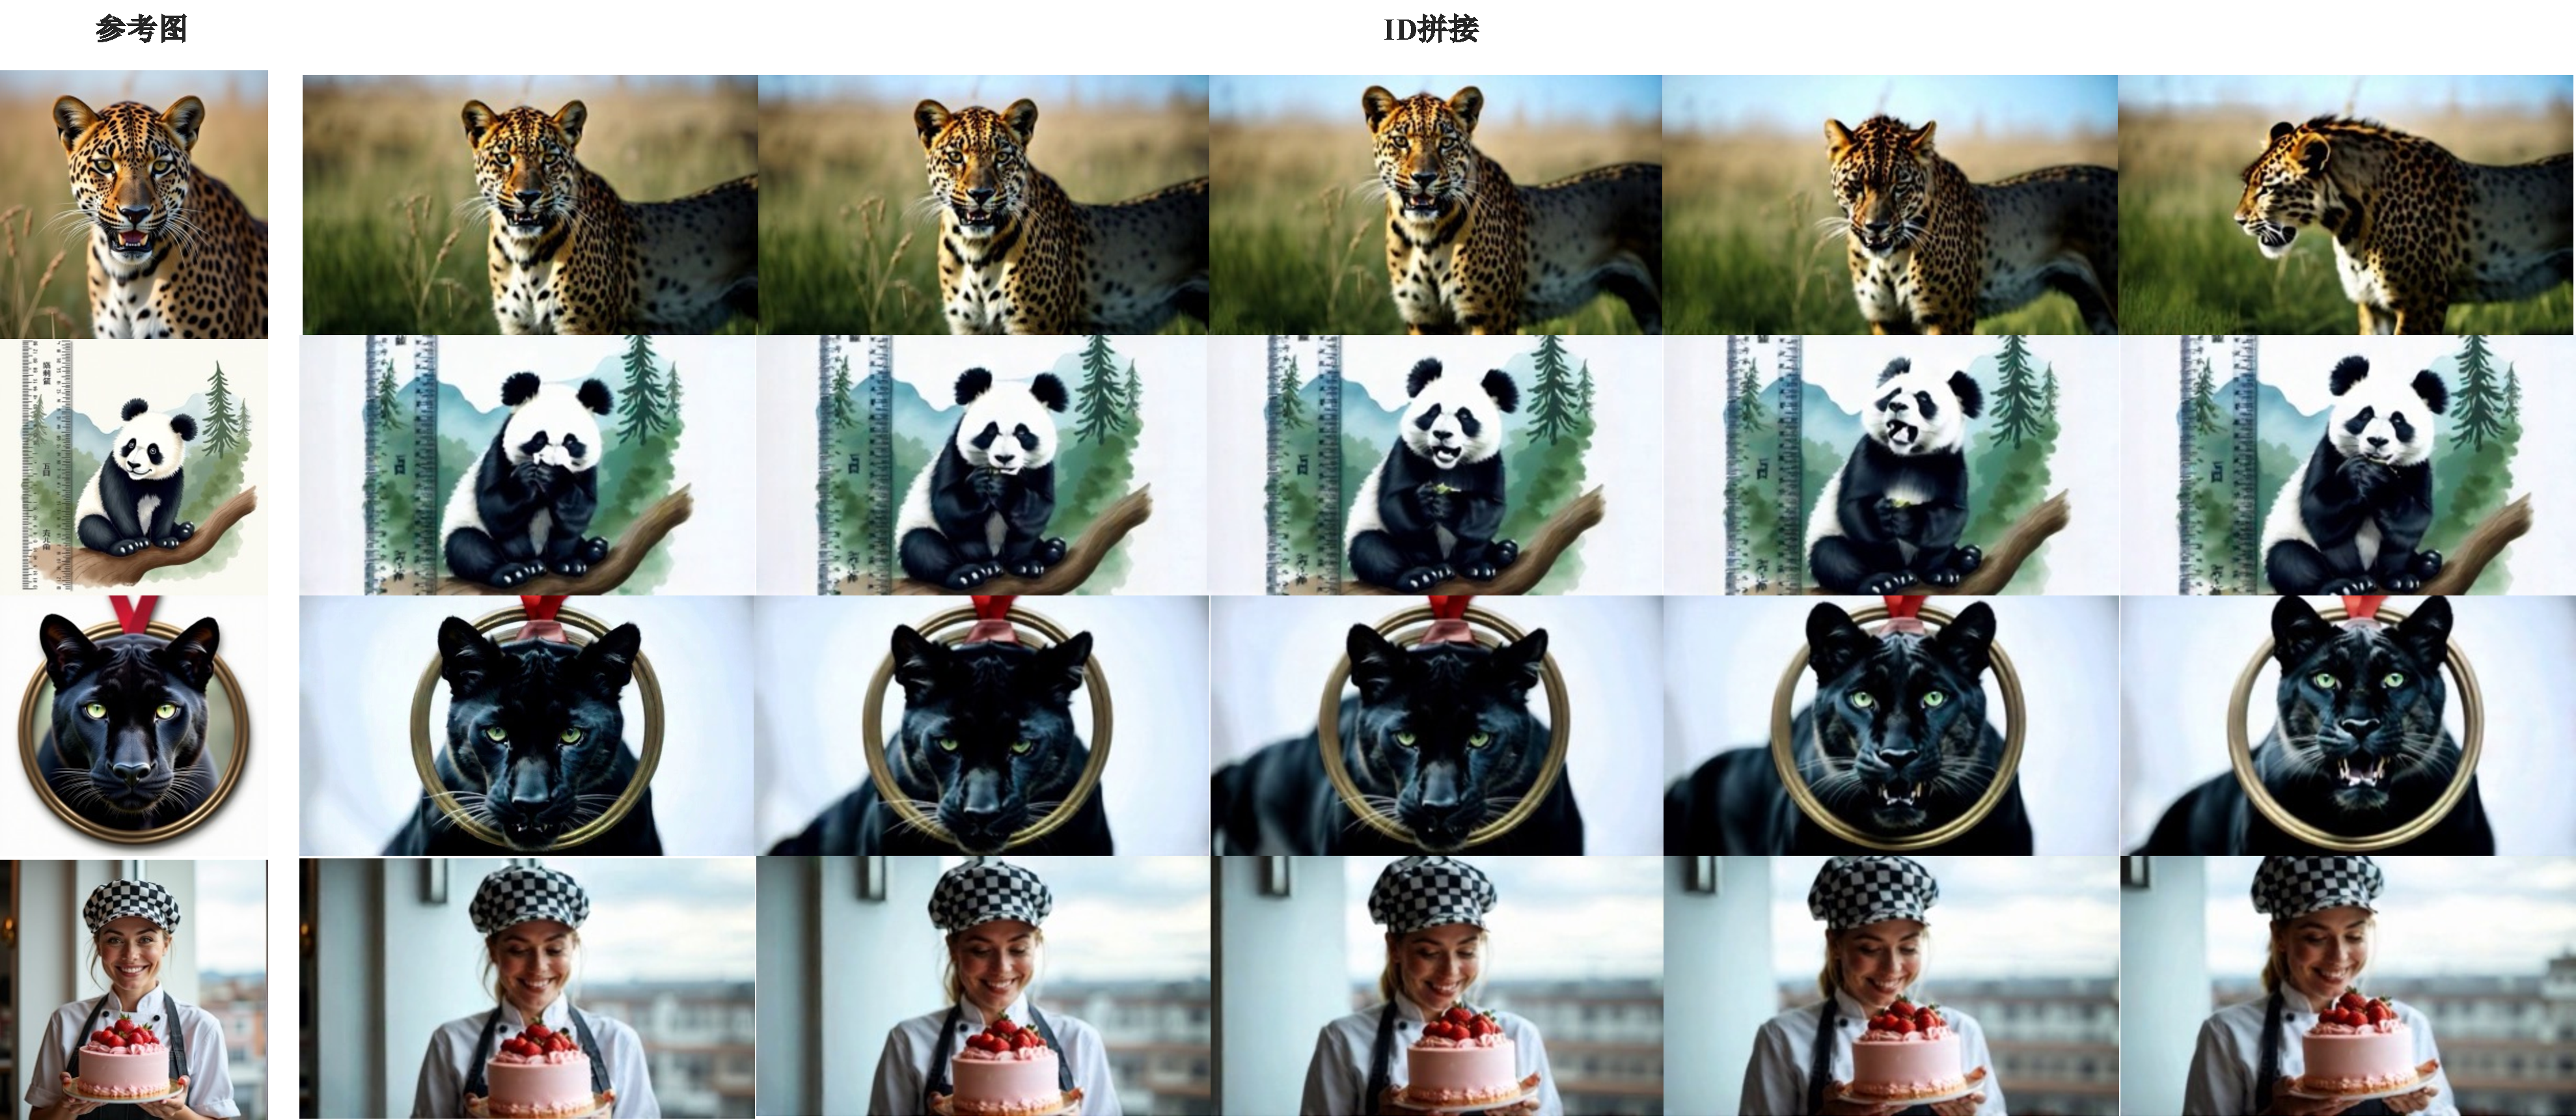
\includegraphics[width=0.8\textwidth]{final/IDconcate_2.pdf}
    \caption{\textbf{}
        注入ID信息视频结果
    }
    \label{IDconcate_2}
\end{figure}
我们还选择涉及到不同动物和人物的案例,如图\ref{IDconcate_2}展示了豹子、熊猫和黑豹和带厨师帽子的女子。这些主体在视频中都表现出了独特的个体特征,既保持了合适的ID信息,同时也进行了相应的视觉变化,确保生成的内容在多个场景下仍能维持一致的身份特征。


\begin{figure}[htbp]
    \centering
    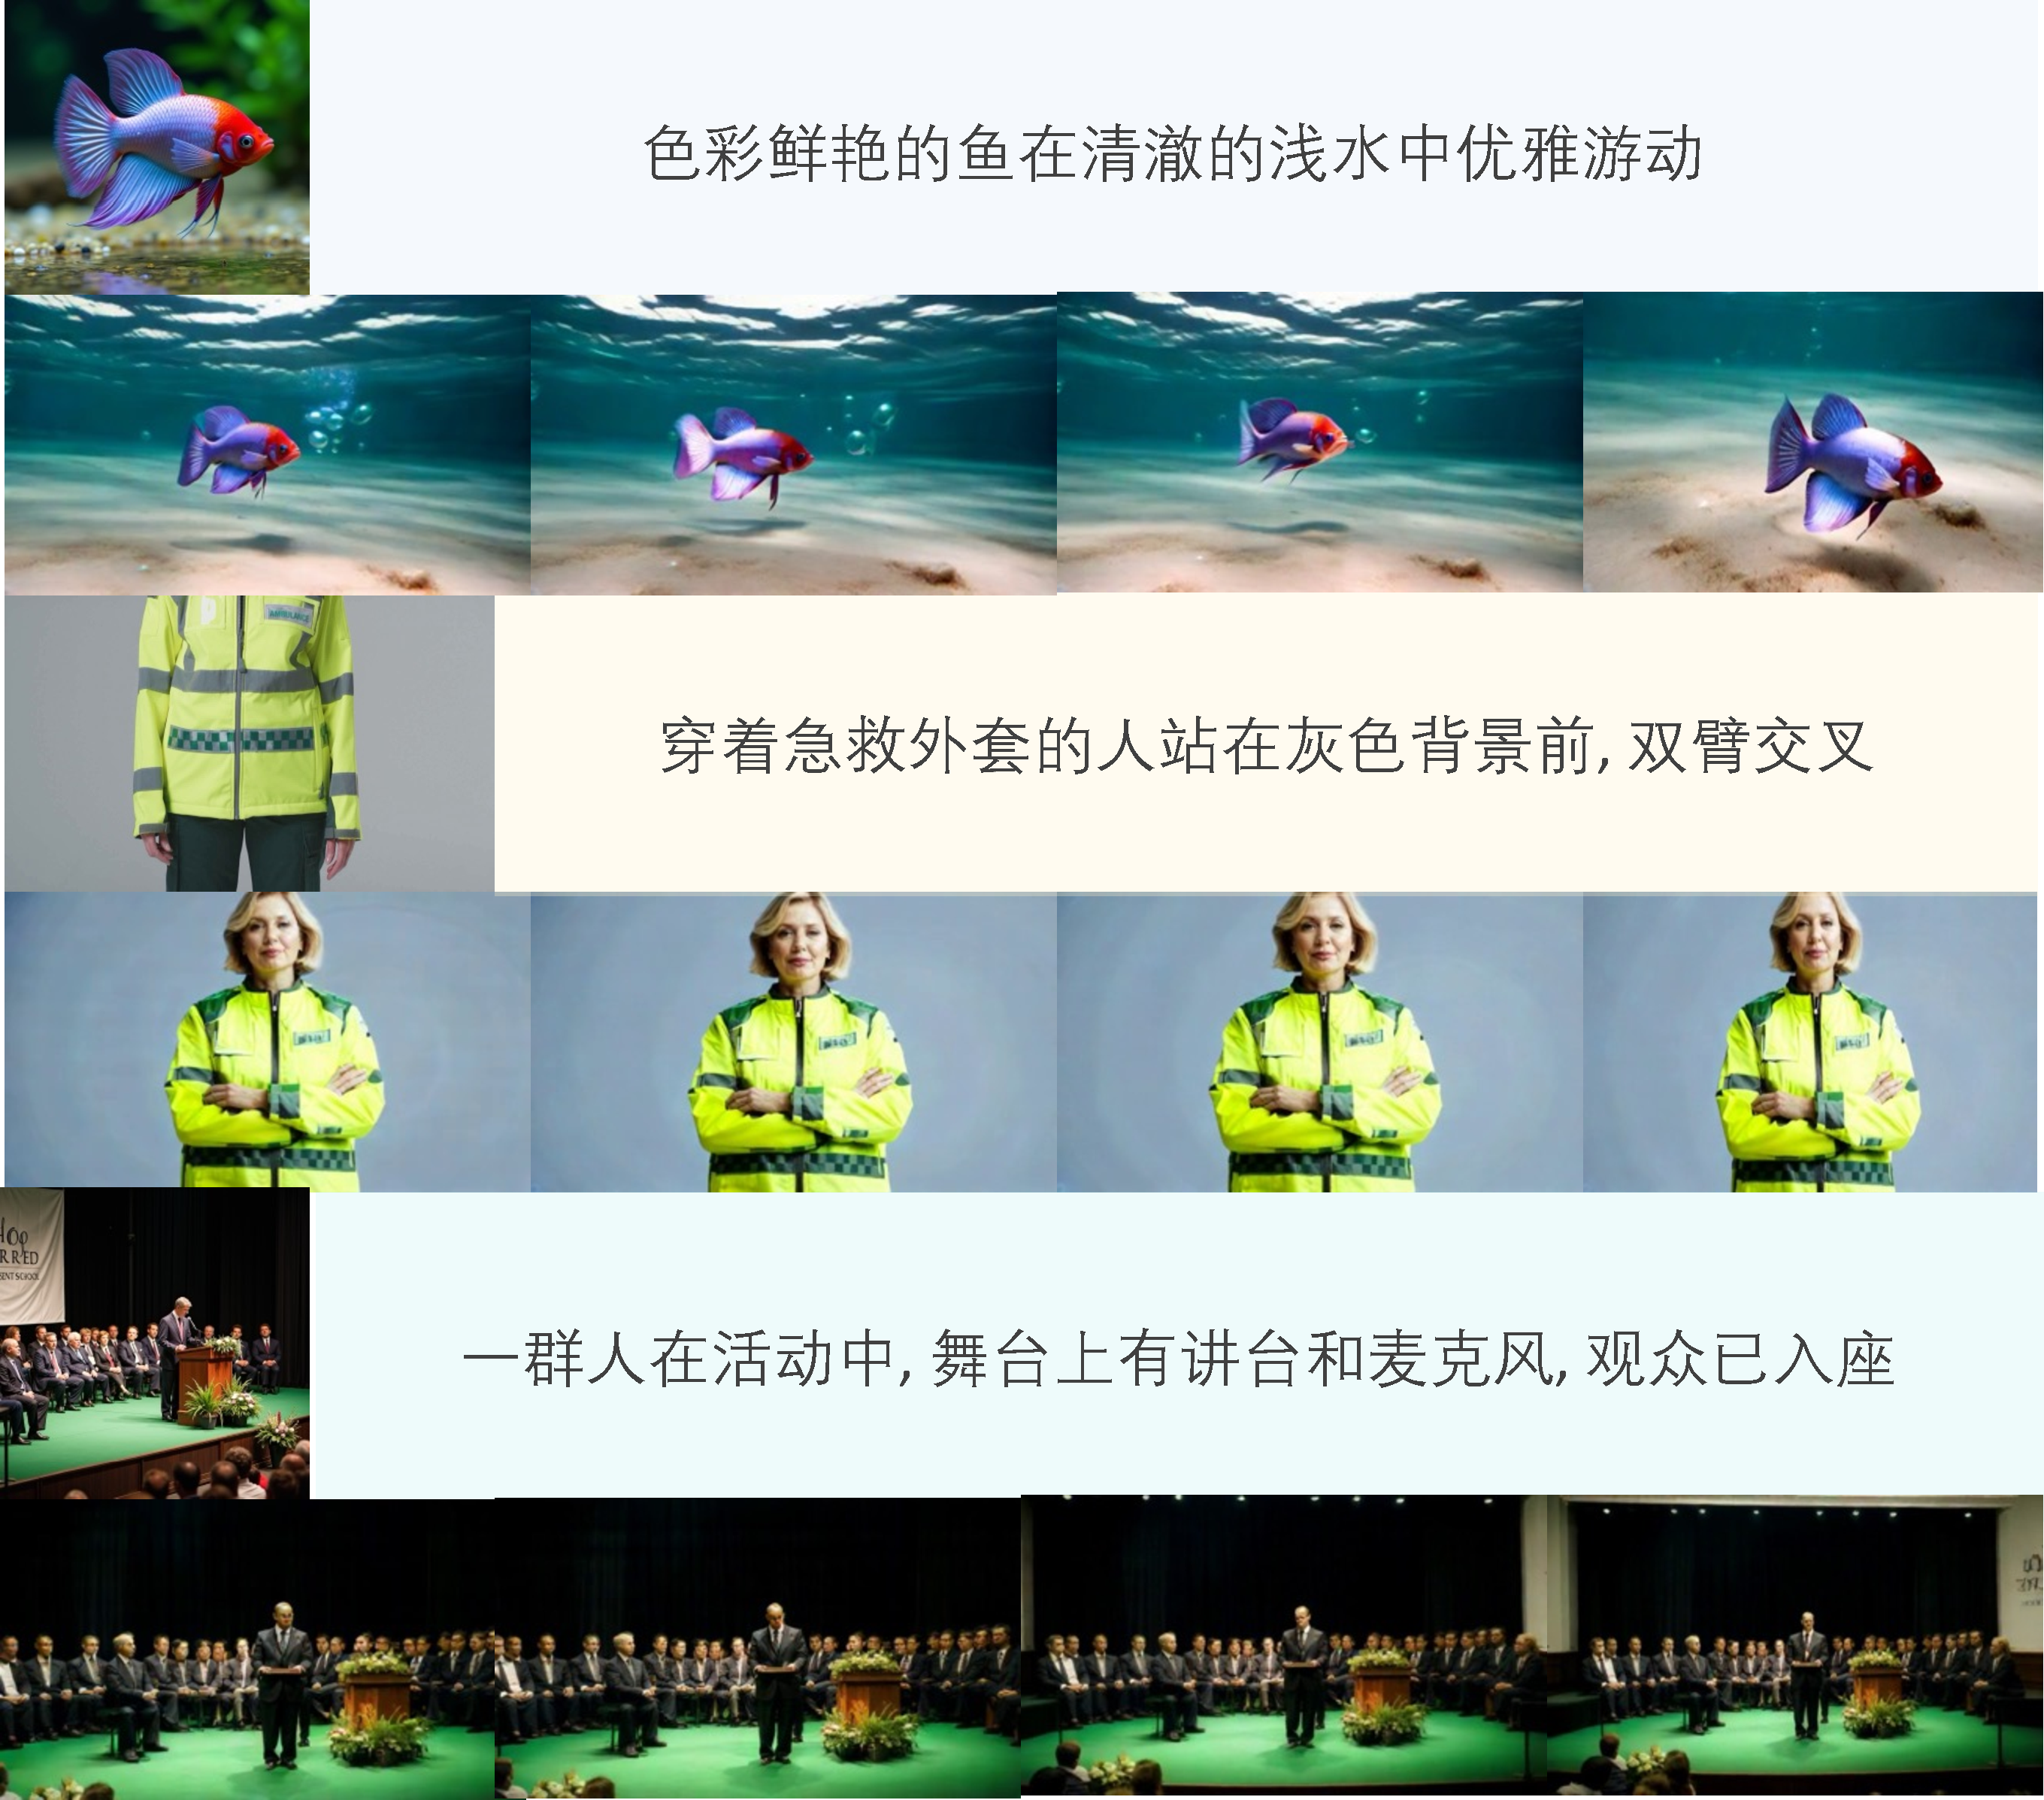
\includegraphics[width=0.8\textwidth]{final/IDconcate_1.pdf}
    \caption{\textbf{}
    注入ID信息视频结果
    }
    \label{IDconcate_1}
\end{figure}
可以看到\ref{IDconcate_1}第一组图像:包含了不同的场景,图像内容包括色彩鲜艳的鱼、穿着急救人员外套的人、以及群体活动的场景。生成的视频动作运动的文本响应度比较高,有较良好的运动状态。而且每个视频都围绕特定的主题进行生成,在保持了人物或场景的发生变动的同时,使得生成的主体内容与给定的参考元素一致。

\begin{figure}[htbp]
    \centering
    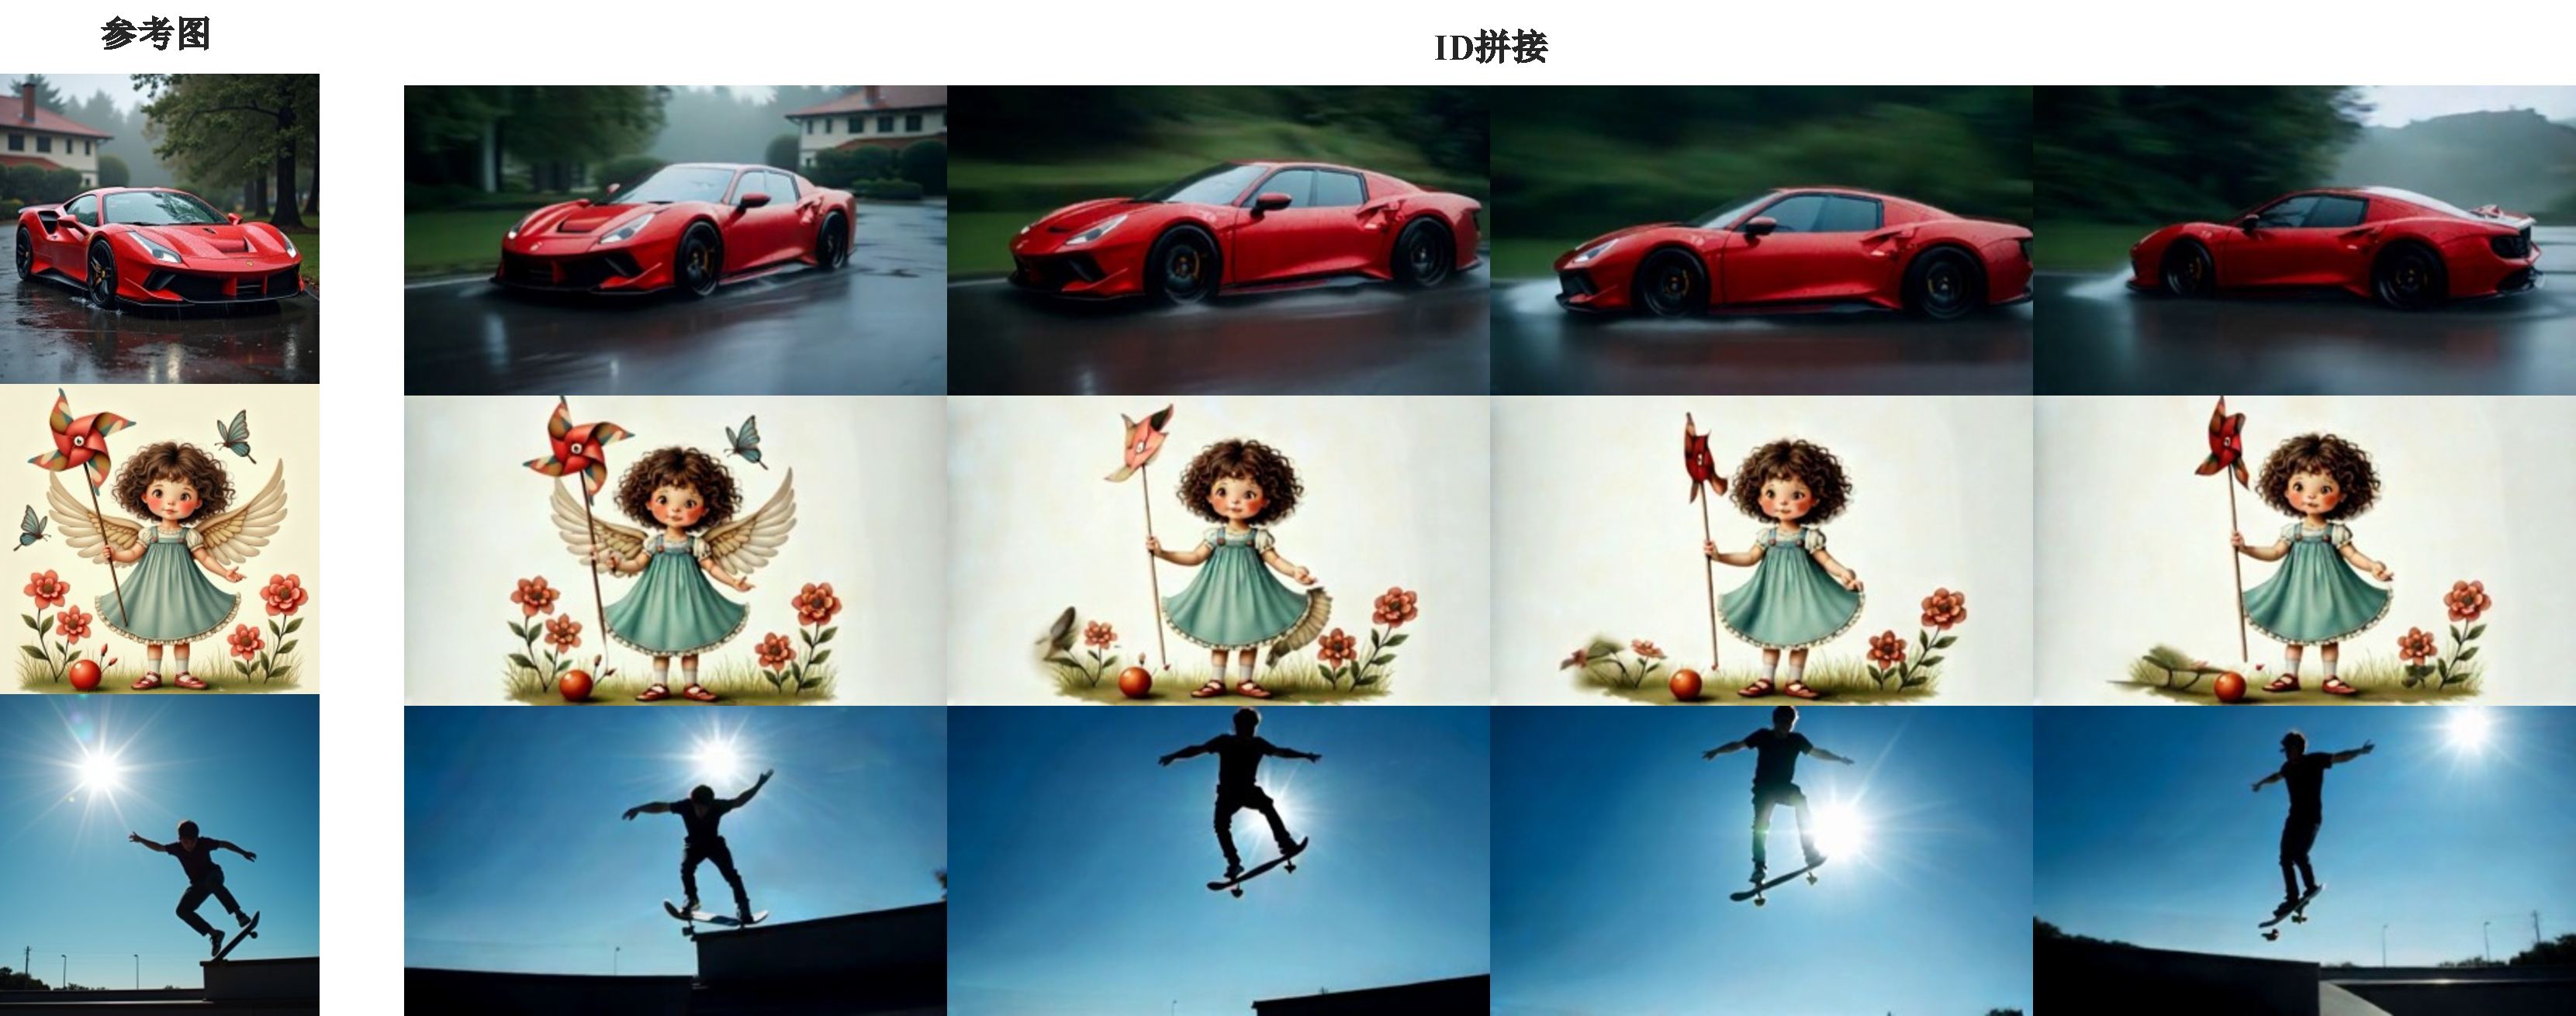
\includegraphics[width=0.8\textwidth]{final/IDconcate_3.pdf}
    \caption{\textbf{}
    注入ID信息视频结果
    }
    \label{IDconcate_3}
\end{figure}
此外对于文本描述词是更大幅度的情况,如飞驰,跳舞和做技巧动作情况,我们也做了相应的实验,如图\ref{IDconcate_3}。视频中的文本响应度也较为良好。对应的文本提示词为(Red sports car speeding through rain, tires splashing in wet street.
一辆红色跑车在大雨中飞驰,轮胎溅起水花,快速行驶在湿滑的街道上。
Whimsical girl with curly hair and wings dancing with pinwheel among flowers.
一位卷发女孩戴着翅膀,在花丛中欢快地跳舞,手持风车。
Skateboarder performing mid-air trick against bright blue sky and sun.
滑板者在明亮蓝天和阳光下空中做技巧动作。
)
基本框架图见图\ref{architecture}
\begin{figure}[htbp]
    \centering
    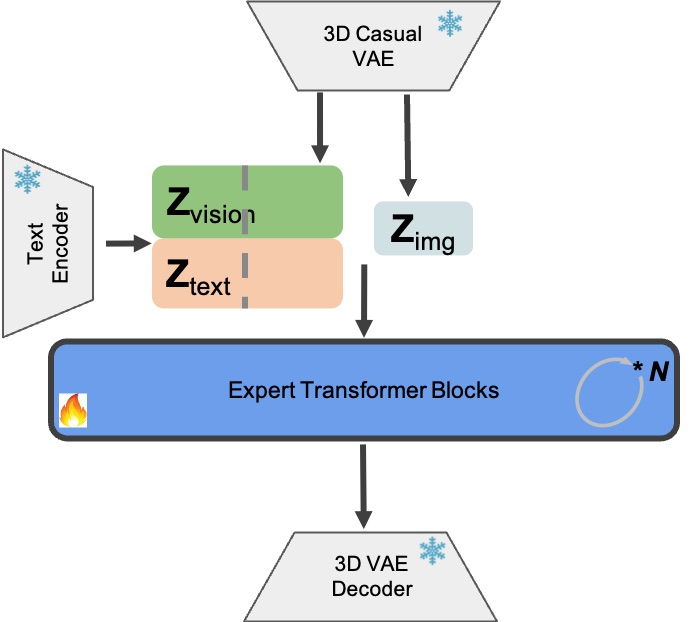
\includegraphics[width=0.8\textwidth]{data3.pdf}
    \caption{\textbf{基于DiT的参考图像生成视频的图片帧拼接策略框架图}
        图像经过VAE编码转化为潜在空间表示(latent space),然后与其他数据进行结合,通过专家Transformer模块进一步处理,并最终解码为视频输出
    }
    \label{architecture}
\end{figure}

此外我们定量测量了VBench指标来评估生成视频的质量。根据表格结果\ref{tab:vbench},我们发现,通过引入额外的信息来保证生成视频的高质量,并且能够保持视频背景的一致性。这种方法能够提供平稳的运动流畅性,但在动态度和美学质量上表现一般。\
首帧替换方法通过将视频的第一帧替换为图像的潜在表示来启动视频生成。这种方法能够在一定程度上保持视频的主题一致性,特别是在人物和背景的细节上有较好表现。然而,这种方法在生成过程中会对动态度产生较大的影响,且美学质量相对较低。\
ID注入方法通过将图像的ID信息注入到生成过程中,使得系统能够更好地保持视频中人物或主体的一致性。尽管它能够增强运动的流畅性和生成的图像质量,但它在动态度和美学质量上的表现较为平淡。ID注入方法的优点在于能够在较少的推理步骤中生成高质量的视频。\
而由于我们所尝试的方法都是在内部的一个小参数(参数量约1B)模型上尝试,所以可以发现和目前最SOTA 模型wan\cite{wan2025}相比,各项指标还有所差异。总结来说Wan视频方法在多数指标上表现优异,尤其是在背景一致性和运动流畅性方面,而ID注入方法则在运动平滑度上表现最为突出。
\begin{table*}[t]
    \centering
    \scriptsize
    \setlength{\tabcolsep}{2pt}
    \renewcommand{\arraystretch}{1.0}
    \resizebox{1\textwidth}{!}{
    \begin{tabular}{l|c|c|c|c|c|c|c|c}
        \toprule
        \textbf{Method} & \textbf{Subject Consistency} & \textbf{Background Consistency} & \textbf{Motion Smoothness} & \textbf{Dynamic Degree} & \textbf{Aesthetic Quality} & \textbf{Imaging Quality} \\ 
        \midrule
        Wan视频 & 92.83 & 95.42 & 98.47 & 54.84 & 62.66 & 69.04 \\
        参考帧拼接 & 93.12 & 95.88 & 98.09 & 45.45 & 62.40 & 62.70 \\
        首帧替换 & 89.22 & 93.53 & 98.81 & 63.64 & 58.25 & 58.09 \\
        \textbf{ID注入} & 95.76 & 95.80 & 99.30 & 37.29 & 57.19 & 58.15 \\
        \bottomrule
    \end{tabular}
    }
    \caption{在VBench指标上比较不同方法的表现}
    \vspace{-0.1in}
    \label{tab:vbench}
\end{table*}

\section{高分辨I2V生成}
\begin{table}[htbp]
    \centering
    \resizebox{1\linewidth}{!}{
    \renewcommand{\arraystretch}{1.2}
    \begin{tabular}{p{2.5cm} p{1.5cm} ccccccc}
    \toprule
    \multirow{2}{*}{\textbf{模型}} & \multirow{2}{*}{\textbf{参数量}} & \multicolumn{7}{c}{\textbf{推理时间 (s/step)}} \\
    \cmidrule(lr){3-9}
     &  & \textbf{49 帧@720p} & \textbf{81 帧@720p} & \textbf{49 帧@1080p} & \textbf{81 帧@1080p} & \textbf{121 帧@1080p} & \textbf{49 帧@2k} & \textbf{81 帧@2k} \\
    \midrule
    CogvideoX & 2B & 4.27 & 9.74 & 32.13 & 79.64 & 171.49 & 95.05 & 248.76 \\
    CogvideoX & 5B & 11.12 & 24.47 & 76.60 & 188.29 & OOM & 225.8 & OOM  \\
    Hunyuan Video & 13B & 11.43 & 29.14 & 98.54 & 258.95 & 552.12 & 326.96 & OOM\\ 
    Wanx Video & 14B & 19.78 & 41.03 & 121.17 & 285.82 & OOM & 341.43 & OOM \\ \midrule
    \textbf{Ours} & \textbf{1B} & \textbf{3.09} & \textbf{4.06} & \textbf{12.35} & \textbf{19.77} & \textbf{34.76} & \textbf{21.12} & \textbf{26.47} \\
    \bottomrule
    \end{tabular}
    }
    \caption{Comparison of model parameters and inference time at different resolution and frames. OOM denotes "out of memory".}
    \label{tab:time_size}
\end{table}


结果前两个部分的探索,已经能够做到生成视频保持参考图基本的主体信息,但是囿于实验模型本身的限制生成一张高分辨率参考图视频会耗费大量的时间,所以我们参考\cite{zhang2025flashvideo
}选择采用reflow 方式。
为了减轻计算开销,我们采用了一个轻量级的流预训练模型,参数为10亿个,能够提高每步去噪效率,如表格~\cref{tab:time_size}所示。
    
该方法在初始化阶段消除了冗余的采样步骤,并避免了对额外控制参数的依赖。在推理过程中,我们从低分辨率的潜变量$\mathbf{lr_latent}$开始,并为了增强模型的生成能力,我们向$\mathbf{lr_latent}$注入噪声,以避免过度依赖其内容。退化过程定义为:
$z_1 = \alpha \cdot \mathbf{lr\_latent} + (1 - \alpha) \cdot \text{noise}, \quad \text{其中} \ \text{noise} \sim \mathcal{N}(0, \mathbf{I})$

然后,我们通过基于常微分方程(ODE)的积分方法,沿着$n$个离散时间步${t_i}{i=0}^n$迭代优化该潜在表示:
$z_1 = z_0 + \sum{i=0}^{n-1} u_\theta(z_{t_i}, t_i) \cdot (t_{i+1} - t_i)$

在训练过程中,我们定义了$z_0$和$z_1$之间的线性插值轨迹:
$z_t = (1 - t) z_0 + t z_1, \quad t \in [0,1]$

然后,真实速度场由下式给出:
$u_{t,\theta} = \frac{dz_t}{dt} = z_1 - z_0$
\begin{figure}[htbp]
    \centering
    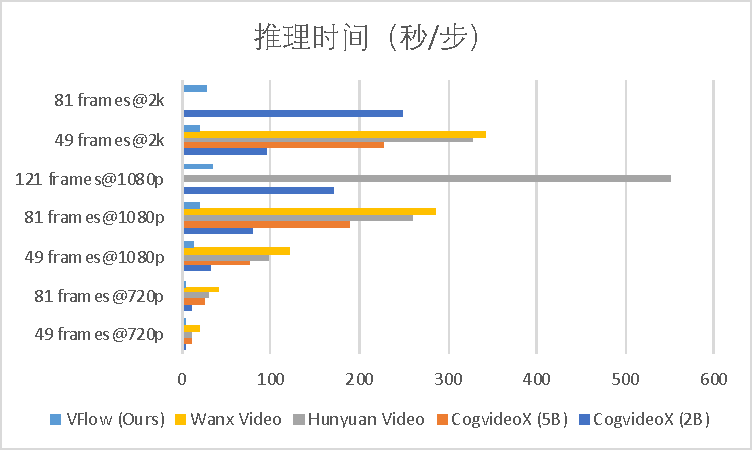
\includegraphics[width=0.8\textwidth]{final/Infer_time_compare.pdf}
    \caption{\textbf{不同模型在不同分辨率和帧数下的推理时间及其模型参数},其中推理时间我们使用推理每步的时长来衡量,单位为秒/步。
    }
    \label{fig:time_size}
\end{figure}
为了建立$\mathbf{lr_latent}$和$\mathbf{hr_latent}$之间的配对关系,我们将$z_0$替换为$\mathbf{hr_latent}$,将$z_1$替换为$\mathbf{lr_latent}$。训练基于流匹配的模型,使得系统能够学习到$\mathbf{lr_latent}$的方向信息,从而在少数推理步骤中生成高质量视频。具体而言,在推理过程中,我们更新$\mathbf{lr_latent}$为:
$z_1 = z_1 - \text{dts}[i] \cdot u_{t,\theta}$。 如簇状条形图\cref{fig:time_size}所示我们比较了我们方法和已有方法之间每步去噪时长差异。展示了不同模型在不同分辨率和帧数下的推理时间及其模型参数。表格中列出了四种模型的推理时间,包括每个模型在多个分辨率(720p、1080p、2k)和不同帧数(49帧、81帧、121帧)下的每步推理时间(单位为秒)。其中,“OOM”表示“内存溢出”,即该配置无法在给定的硬件条件下完成推理。

具体而言,模型 CogvideoX(2B参数量)在49帧720p分辨率下的推理时间为4.27秒,而在81帧2k分辨率下则为248.76秒。对于更大参数量的 CogvideoX(5B),推理时间在各分辨率和帧数下明显增加,尤其在121帧1080p分辨率时出现内存溢出。

与之相比,我们的方法,1B参数量在所有配置下的推理时间表现较优,特别是在49帧720p和81帧720p分辨率下,其推理时间分别为3.09秒和4.06秒,显著低于其他模型。我们修改方案的推理时间在其他高分辨率下也保持较好的性能,如49帧2k分辨率时为21.12秒,81帧2k分辨率时为26.47秒。

该表格通过对比展示了不同模型在推理效率上的差异,表明我们方法在资源有限的条件下,能够提供更高效的推理表现。

\begin{figure}[htbp]
    \centering
    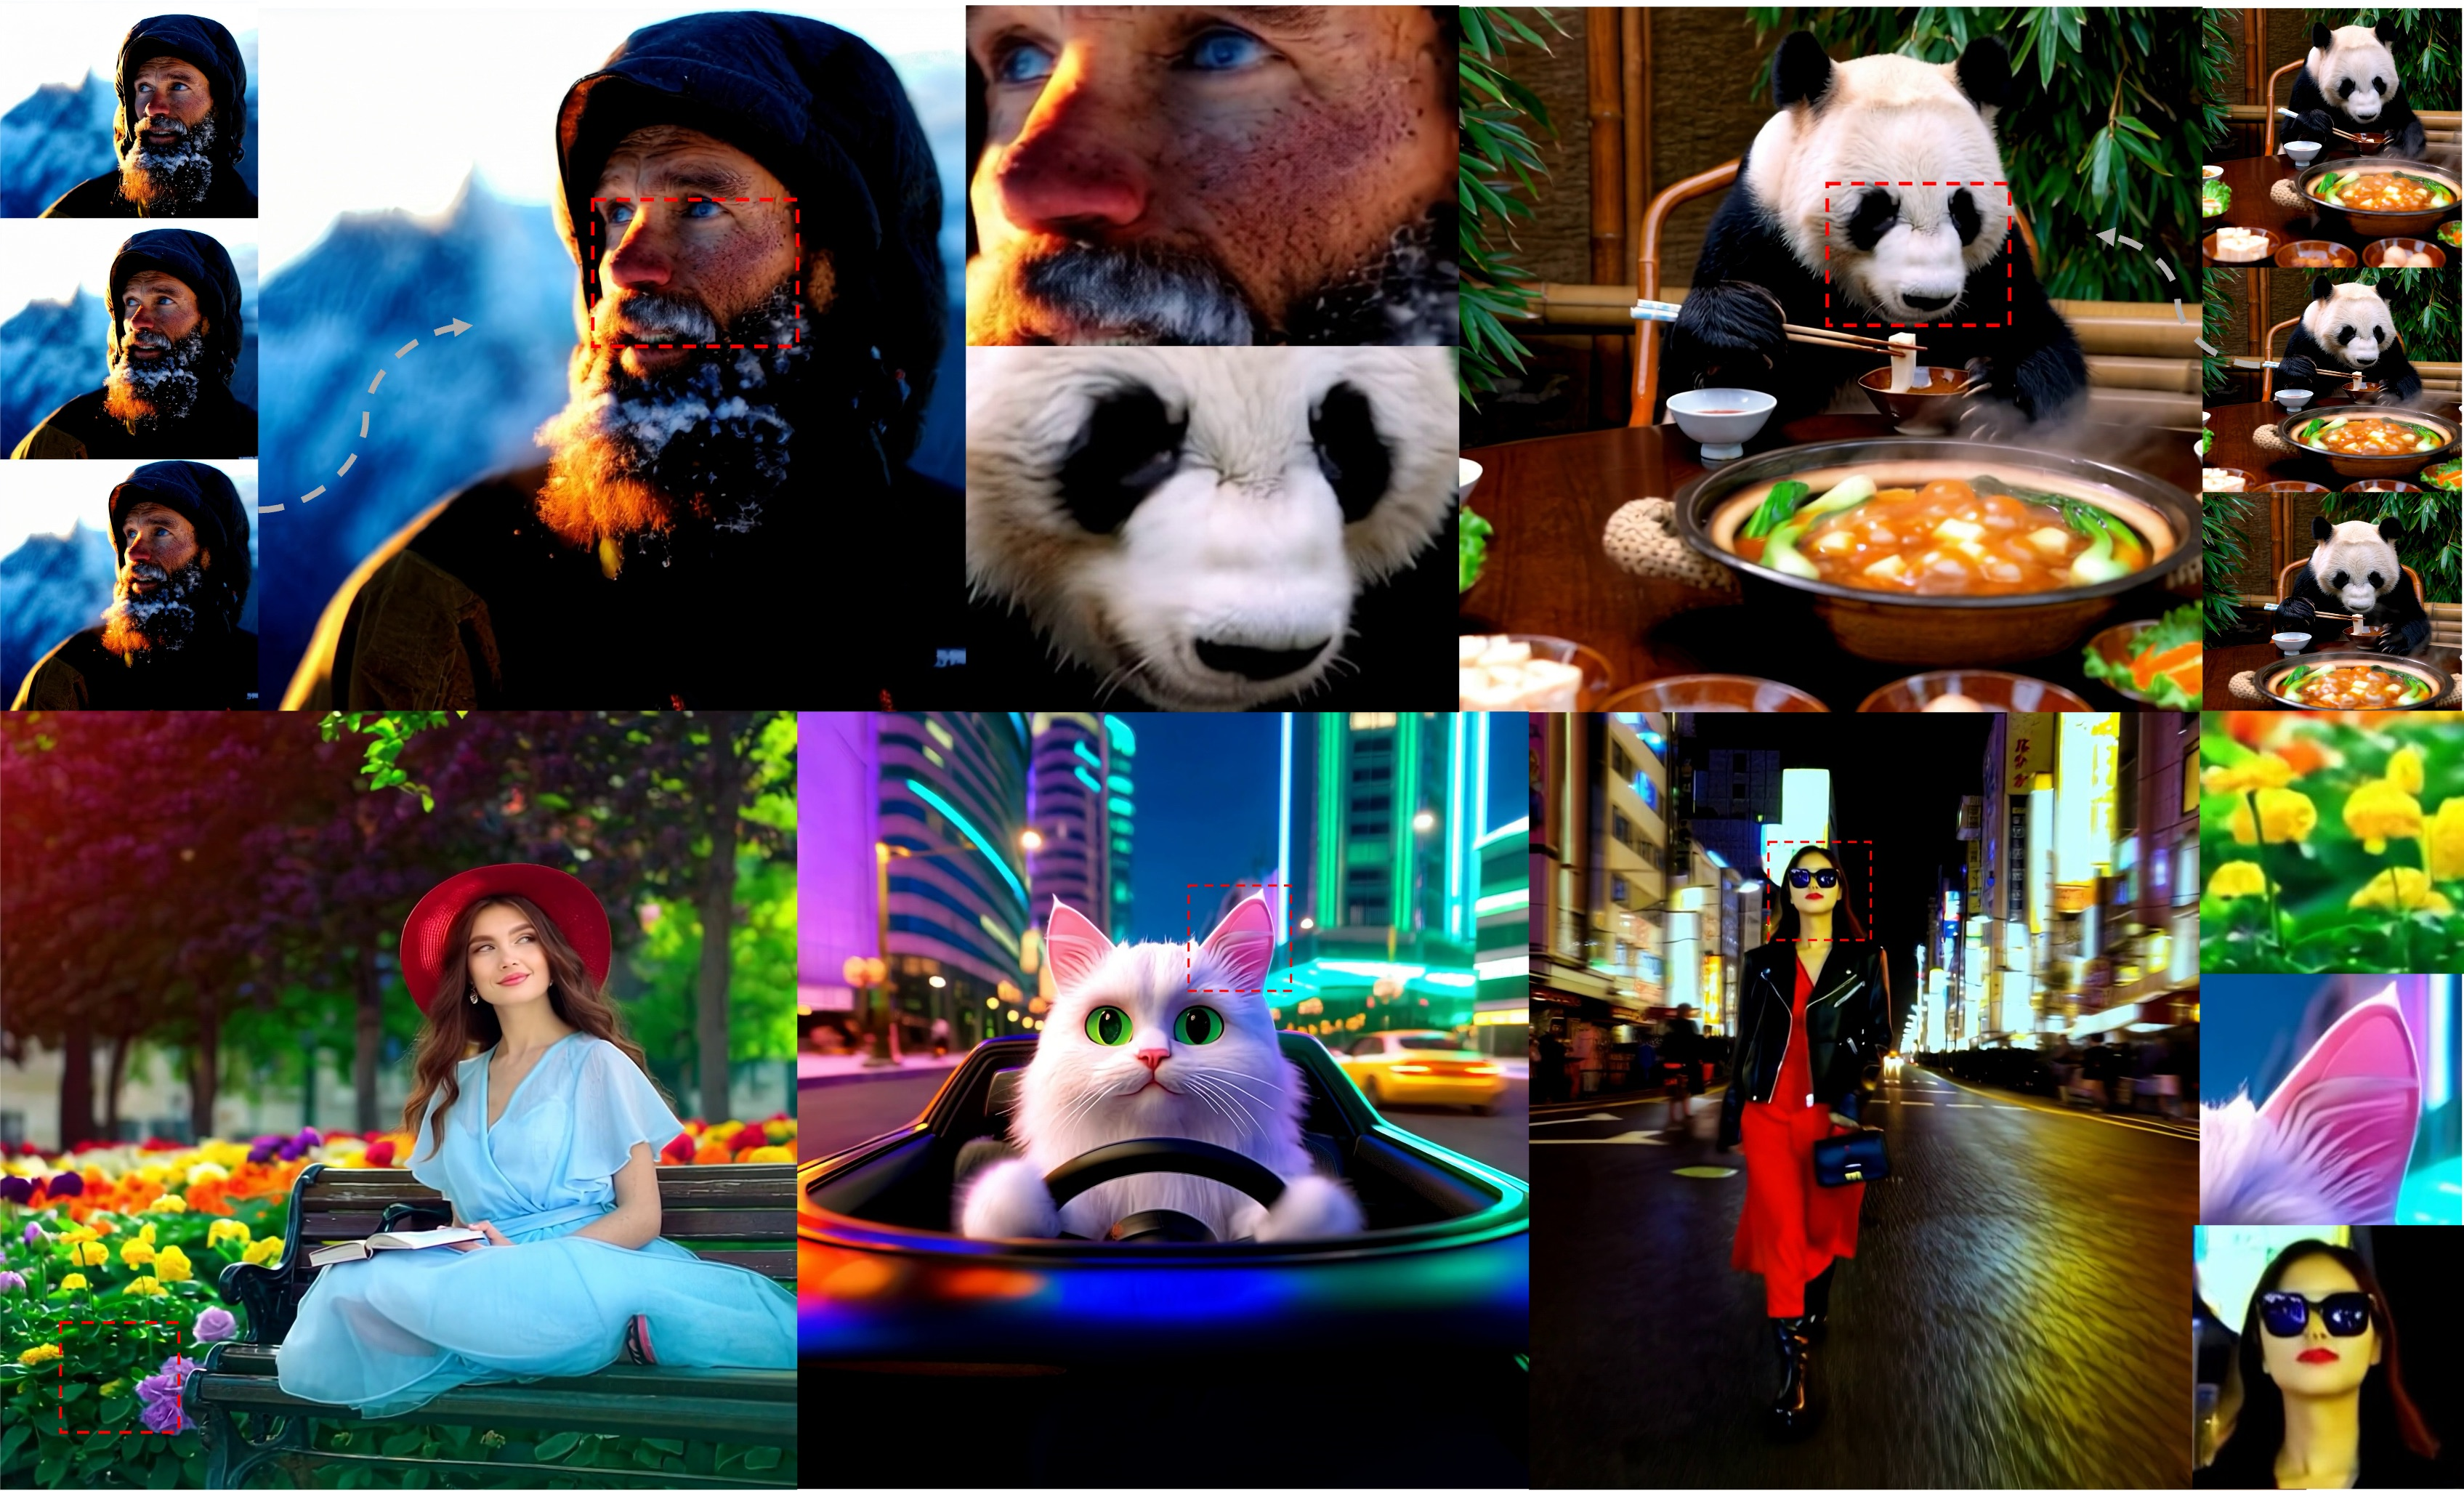
\includegraphics[width=0.8\textwidth]{final/hqvideo.pdf}
    \caption{
        \textbf{高分辨率视频生成结果展示}
    }
    \label{hqvideo}
\end{figure}

\section{未来展望}
